\documentclass[11pt]{article}

\usepackage[T1]{fontenc}
\usepackage[utf8]{inputenc}
\usepackage{lmodern}
\usepackage[margin=1in]{geometry}
\usepackage{amsmath,amssymb,amsthm,mathtools}
\usepackage{booktabs}
\usepackage{tabularx}
\usepackage{graphicx}
\usepackage{placeins}
\usepackage{float}
\usepackage{enumitem}
\usepackage{fontawesome5}
\usepackage{microtype}
\usepackage{xspace}
\usepackage{xcolor}
\usepackage{hyperref}
\usepackage[round,authoryear]{natbib}
\usepackage{tikz}
\usetikzlibrary{arrows.meta,positioning,fit}

\hypersetup{
  colorlinks=true,
  linkcolor=black,
  citecolor=blue!55!black,
  urlcolor=blue!55!black,
  pdftitle={TreeWork: State-Native Project Memory for Long-Horizon Coding Agents},
  pdfauthor={Zhongxuan Song}
}

\setlist{nosep,leftmargin=*}
\newcommand{\system}{\textsc{TreeWork}\xspace}
\newcommand{\M}{\mathcal{M}}
\newcommand{\Z}{\mathcal{Z}}
\newcommand{\B}{\mathcal{B}}
\newcommand{\G}{\mathcal{G}}
\newcommand{\T}{\mathcal{T}}
\newcommand{\D}{\mathcal{D}}
\newcommand{\E}{\mathcal{E}}
\newcommand{\A}{\mathcal{A}}
\newcommand{\K}{\mathcal{K}}
\newcommand{\Lset}{\mathcal{L}}
\newcommand{\Vset}{\mathcal{V}}
\newcommand{\Recall}{\operatorname{Recall}}
\newcommand{\Apply}{\operatorname{Apply}}
\newcommand{\Valid}{\operatorname{Valid}}
\newcommand{\TopK}{\operatorname{TopK}}
\newcommand{\Read}{\operatorname{Read}}

\newtheorem{theorem}{Theorem}[section]
\newtheorem{lemma}[theorem]{Lemma}
\newtheorem{proposition}[theorem]{Proposition}
\newtheorem{corollary}[theorem]{Corollary}
\theoremstyle{definition}
\newtheorem{definition}[theorem]{Definition}

\title{\system: State-Native Project Memory for Long-Horizon Coding Agents}

\author{Zhongxuan Song\\
\small University of Science and Technology of China\\
\texttt{universeszym@mail.ustc.edu.cn}\\
\small\href{https://github.com/Johnny-xuan/TreeWork}
{\textcolor{black}{\faGithub\ \texttt{Code}}}}
\date{}

\begin{document}
\maketitle

\begin{abstract}
Long-horizon coding agents lose operational coordination state across context
compression, interruptions, task switching, and handoffs between agents.
Most external agent-memory systems are retrieval-native: they store textual
facts, episodes, reflections, or trajectories and later retrieve a small set of
items relevant to a query.  Coding agents can also inspect the repository, but
a finite context budget permits only a partial view of a large codebase, and
source code primarily records implementation outcomes rather than the accepted
intent and process that produced them.  Retrieval and code inspection are both
necessary, but machine-owned coordination state is a different object.
Continuing software work requires a complete and current account of fields such
as which branch owns a request, which dependencies are satisfied, and what
verification is still missing, together with governed references to the
accepted design.  TreeWork treats the structured fields as authoritative; it
does not assume that narrative artifacts are automatically complete or correct.

We present \system, a state-native project memory system for coding agents.
\system represents a project as an ordered rooted Project Tree augmented by a
dependency DAG, branch-local Specs and execution documents,
machine-owned lifecycle state, verification evidence, and a compact event
trajectory of accepted state transitions.  Rather than reconstructing state
from semantically similar fragments, \system exposes deterministic projections
for branch recall, current project visualization, and trajectory replay.  Its
three-stage protocol---Pre-Tree Alignment, Build Tree, and Work
Tree---separates intent formation, state-space construction, and branch-local
execution.  A transaction layer validates structural and lifecycle changes and
publishes them through a marker-defined logical commit, while Git worktrees
isolate branch execution.

We formalize the observation--state reconstruction gap, the \system machine-state
model, its admissible transition relation, and its query projections.  We prove
a continuation-error lower bound for decisively aliased observations and give
conditional sufficiency and soundness guarantees for guard-complete projections
and marker-consistent committed reads.  We also describe the implemented system and
specify an evaluation protocol for measuring state-recovery accuracy,
trajectory drift, handoff cost, development quality, and workflow overhead.
Accordingly, this paper focuses on the system design, formal properties, and a
reproducible protocol for controlled evaluation.
\end{abstract}

\section{Introduction}

Coding agents increasingly navigate repositories, edit files, execute tools,
and verify changes rather than merely generate isolated code snippets
\citep{yang2024sweagent,jimenez2023swebench}.  Their work is therefore
sequential and stateful.  A meaningful project may span many modules, design
decisions, interrupted sessions, context-window compressions, and human or
multi-agent handoffs.  At each continuation point, the acting agent must know
not only what was said in the past, but where the project currently is.

Repository inspection is indispensable for grounding an agent in implementation
reality.  Source files, tests, and existing documentation reveal what the
system currently does.  They do not, however, provide a cheap or unique inverse
of the development process.  A large repository can only be sampled under a
finite context budget; several design histories may yield similar code; and
source code does not reliably identify which requirements were accepted, which
alternatives were rejected, whether a module is complete or merely paused, or
which evidence is still required.  Git preserves physical change history, but
diffs do not by themselves encode the accepted semantic trajectory of the
project.

External memory is a common response to context limits.  Representative systems
store observations or reflections and retrieve relevant items for future
reasoning \citep{park2023generative,shinn2023reflexion}; others manage memory
tiers \citep{packer2023memgpt}, build linked note networks
\citep{xu2025amem}, or evolve reusable contexts
\citep{zhang2025ace}.  These approaches make valuable past information
available, but they generally frame reading as a relevance problem: given a
query, which stored fragments should enter the next context?

Project continuation poses a stricter problem.  Suppose an agent retrieves one
old statement that branch $b$ is blocked, one newer note that its dependency
was completed, and a design discussion that was later superseded.  All three
items may be semantically relevant.  None alone identifies the authoritative
current state.  A top-$k$ retriever may omit a necessary dependency, return a
stale decision, or present conflicting memories without an update rule.  Recent
work has independently found a gap between retrieving updated evidence and
acting on the resulting state \citep{chao2026stale}.  More generally, surveys of
agent memory identify contradiction handling, continual consolidation, and
causally grounded retrieval as open problems \citep{du2026memory}.

We call this mismatch the \emph{observation--state reconstruction gap}.  The
problem is neither repository inspection nor retrieval itself.  The problem is
asking an agent to reconstruct authoritative current state from a partial view
of implementation outcomes plus semantically relevant historical fragments.
For project continuation, code inspection should remain the source of
implementation truth, while coordination state should be an exact projection
of maintained machine-owned project state.  Semantic retrieval can remain
supplementary.

\system addresses this gap for long-horizon software development.  It
externalizes persistent project memory in which:

\begin{itemize}
  \item a rooted tree defines hierarchical work ownership;
  \item a dependency DAG constrains feasible ordering and parallelism;
  \item project- and branch-scoped Specs preserve technical design
        formed before coding;
  \item Plans, Progress, Findings, and Verification records separate intended
        work, current reality, learned conclusions, and completion evidence;
  \item lifecycle transactions maintain branch position and status;
  \item a compact semantic event stream preserves the accepted development
        trajectory; and
  \item deterministic read models let agents and humans recover the same
        accepted coordination state.
\end{itemize}

\system is not a fixed workflow engine and does not execute or schedule agents.
A fixed workflow typically provides a policy or prescribed control flow over
steps.  \system instead defines a shared state space and an admissible
transition relation.  The agent retains freedom over local implementation and
branch choice, subject to explicit ownership, design, dependency, verification,
and transition constraints.  In this sense, the system supports
\emph{trajectory engineering}: it makes the path of long-running development
explicit, recoverable, and inspectable without prescribing every action.

\begin{figure}[htbp]
\centering
\includegraphics[width=\textwidth]{assets/two_panel_agent_workflow_comparison_4k_final.png}
\caption{Repository inspection and memory retrieval expose implementation
outcomes and historical fragments, but leave the agent to reconstruct current
coordination state.  TreeWork retains targeted code inspection and optional
retrieval while exposing accepted coordination state through a deterministic
projection.}
\label{fig:memory-comparison}
\end{figure}
\FloatBarrier

Our contributions are:

\begin{enumerate}
  \item We formulate the observation--state reconstruction gap for
        long-horizon coding work and distinguish partial repository inspection
        plus relevance-oriented recall from authoritative project-state
        recovery.
  \item We define state-native project memory as a composition of accepted
        structured state, scope-owned documents, semantic transition events,
        and deterministic query projections.
  \item We introduce the \system methodology: a three-stage development
        protocol over an ordered Project Tree and dependency DAG, with
        specification-first branches, protected lifecycle transitions, and
        verification-gated completion.
  \item We prove a continuation-error lower bound under decisively aliased
        observations and establish conditional sufficiency and committed-state
        soundness results for explicit coordination projections.
  \item We describe a working implementation as a coding-agent plugin with a
        Rust transaction runtime, Git worktree isolation, branch recall, and
        read-only Map, Dependency, and Replay views.
  \item We provide a reproducible evaluation protocol for measuring state
        recovery, trajectory drift, handoff cost, development quality, and
        workflow overhead.
\end{enumerate}

\section{Related Work}

\subsection{Retrieval-Augmented and Agent Memory}

Retrieval-augmented generation combines parametric generation with retrieved
external evidence \citep{lewis2020rag}.  Memory-augmented language agents further
distinguish working context from semantic, episodic, or procedural memory
\citep{sumers2023coala,du2026memory}.  Generative Agents retrieve experiences
and reflections \citep{park2023generative}; Reflexion retains verbal feedback
across trials \citep{shinn2023reflexion}; MemGPT manages hierarchical memory
tiers \citep{packer2023memgpt}; A-MEM evolves linked notes
\citep{xu2025amem}; and ACE curates an evolving context playbook
\citep{zhang2025ace}.

These systems preserve knowledge, experience, and reusable strategy.  \system
defines a different read contract: not which historical items are relevant to
a query, but which operational state is currently accepted for a named branch.
Retrieval remains complementary evidence; it does not by itself provide
authority, supersession, or a deterministic current-state projection.

\subsection{Stateful Workflows and Formal Transition Systems}

ReAct interleaves reasoning and actions \citep{yao2023react}, while StateFlow
uses state-driven workflows to ground task execution \citep{wu2024stateflow}.
Earlier systems traditions already supply the formal machinery that TreeWork
uses: Statecharts model hierarchical and concurrent state
\citep{harel1987statecharts}; TLA+ specifies behavioral properties of discrete
systems \citep{lamport2002specifying}; linearizability formalizes the appearance
of atomic concurrent operations \citep{herlihy1990linearizability}; and
transaction processing develops atomic commit, logging, and recovery
\citep{gray1992transaction}.  TreeWork applies these established mechanisms to
durable coding-project state and asks an additional question:
which projected fields are sufficient to determine admissible continuation
movements?

Agent trajectories are also studied as first-class analysis objects.  In
software engineering, thought--action--result trajectories expose recurring
motifs, costs, and failures \citep{bouzenia2025trajectories}.  TreeWork stores a
coarser semantic trajectory containing accepted project transitions rather than
private reasoning, raw shell history, or source diffs.  Its state persists
across tasks and agents without selecting the next tool call or executing an
LLM workflow graph.

\subsection{Event-Sourced State, Provenance, and Decision Records}

Event Sourcing represents application changes as an event sequence that can
explain or reconstruct state \citep{fowler2005eventsourcing}.  W3C PROV models
entities, activities, agents, and derivation for provenance interchange
\citep{lebo2013provo}.  Architecture Decision Records preserve decision context,
status, consequences, and supersession \citep{nygard2011adr}.  These traditions
cover complementary questions: what happened, how an artifact was produced,
and why a design was accepted.

TreeWork combines a narrower typed event trajectory with branch-local design
and current lifecycle state to answer what a branch permits now.  It is not a
pure event-sourced read model: current Project Map and Recall projections read
materialized committed state, while events and checkpoints support historical
Replay.  Git remains the source of file-level provenance.

\subsection{Software Project Coordination and Acceptance Infrastructure}

Production software platforms already maintain substantial authoritative
coordination state.  GitHub Issues supports nested work and blocking
dependencies \citep{github2026issues}; protected branches can require reviews,
status checks, resolved conversations, successful deployments, and merge queues
\citep{github2026protected}.  Modern code review likewise combines technical
inspection with a social acceptance process \citep{sadowski2018review}.

Work hierarchies, dependencies, and completion gates are established
coordination mechanisms, but their state is often distributed across issues,
pull requests, CI, documents, and Git.  TreeWork organizes the subset needed to
continue coding as a branch-scoped contract connecting accepted design,
lifecycle, verification, deterministic reads, and guarded writes.

\subsection{Multi-Agent Coordination and Shared State}

Blackboard architectures established shared external state as a coordination
medium for heterogeneous knowledge sources \citep{hayesroth1985blackboard}.
Contemporary LLM systems explore complementary message- and workflow-oriented
coordination: AutoGen centers programmable multi-agent conversation
\citep{wu2023autogen}; MetaGPT encodes roles and standard operating procedures
\citep{hong2023metagpt}; and ChatDev structures software development through
communicative agents and chat chains \citep{qian2024chatdev}.

TreeWork does not replace inter-agent communication, allocate workers, or run a
team.  It supplies shared committed domain state so that handoffs need not
retransmit project location, accepted design, lifecycle, and completion evidence
only through messages.  Coordination through shared state and coordination
through communication remain complementary.

\subsection{Agent Interfaces and Domain-Specific State Systems}

SWE-bench exposes the difficulty of repository-level issue resolution
\citep{jimenez2023swebench}, and SWE-agent demonstrates that an agent-computer
interface materially changes coding-agent behavior \citep{yang2024sweagent}.
TreeWork extends this interface perspective from code manipulation to recovery
of project coordination state.

Other agent domains reinforce that action-relevant state is domain-specific.
WebArena and OSWorld define reproducible web and desktop environments with
task-specific initial state and executable outcomes
\citep{zhou2023webarena,xie2024osworld}; Voyager combines embodied exploration,
environment feedback, and a growing skill library \citep{wang2023voyager}; and
The AI Scientist spans idea formation, experiments, artifacts, and review
\citep{lu2024aiscientist}.  These are not interchangeable state-memory systems.
They motivate the broader view that coding, GUI, embodied, and research agents
require different state schemas connected by common projection interfaces.

Across these traditions, the components of TreeWork are individually familiar.
Its system contribution is their combination into a coding-agent-facing,
branch-scoped deterministic continuation projection, linked to authority and
supersession, admissible movements, transactional writes, and agent-independent
handoff.

\section{Problem Formulation}
\label{sec:problem}

\subsection{Partial Repository Observation and Retrieval}

Let $X_t$ be the complete repository snapshot at time $t$, let
$H_t=\{m_1,\ldots,m_n\}$ be available memory items, and let $q_t$ be a query
derived from the agent's current context.  Under a context budget $\beta$, an
agent obtains a local repository observation

\begin{equation}
  O_\beta(q_t,X_t)\subseteq X_t.
  \label{eq:repository-observation}
\end{equation}

It may also retrieve semantically relevant memory:

\begin{equation}
  R_k(q_t,H_t)
  =
  \TopK_{m\in H_t}\; \operatorname{sim}(q_t,m),
  \label{eq:retrieval}
\end{equation}

followed by a model-dependent reconstruction

\begin{equation}
  \widehat{z}_t
  =
  f_\theta\!\left(
    q_t,
    O_\beta(q_t,X_t),
    R_k(q_t,H_t)
  \right),
  \label{eq:reconstruction}
\end{equation}

where $z_t$ denotes the operational state required to continue work.
Repository tools select files relevant to the current query, while
Equation~\ref{eq:retrieval} optimizes memory relevance.  Neither operation
directly optimizes global state validity.  Without additional machinery, their
combination provides no guarantee that the reconstructed state is:

\begin{itemize}
  \item \emph{complete}: all required dependencies and constraints are present;
  \item \emph{current}: superseded facts are excluded;
  \item \emph{authoritative}: conflicts are resolved according to an accepted
        write path;
  \item \emph{causally situated}: the reasons and transitions leading to the
        current state are preserved; or
  \item \emph{actionable}: the next admissible project movement is identifiable.
\end{itemize}

For a state-distance function $d$, define the reconstruction error as

\begin{equation}
  \Delta_t = d(\widehat{z}_t,z_t).
  \label{eq:state-gap}
\end{equation}

Increasing $k$ or the context window may reduce omission, but it does not by
itself define supersession, authority, lifecycle, or admissible transitions.

There is also an information problem independent of context size.  Let
$h_t=(Q_t,S_t,\widetilde{\tau}_t)$ denote accepted Requirements, Spec, and
semantic development trajectory, and let $\alpha_{\leq t}$ denote physical
implementation actions.  A repository snapshot is produced by some development
map

\begin{equation}
  X_t=\Psi(h_t,\alpha_{\leq t}).
  \label{eq:repository-result}
\end{equation}

This map is generally not injective:

\begin{equation}
  \exists (h,\alpha)\neq(h',\alpha')
  \quad\text{s.t.}\quad
  \Psi(h,\alpha)=\Psi(h',\alpha').
  \label{eq:non-injective-code}
\end{equation}

Different accepted intentions, rejected alternatives, pauses, and verification
histories can yield the same or observationally equivalent source snapshot.
Code is therefore necessary evidence of implementation reality, but it is not
a lossless encoding of project process.

\subsection{State-Native Read Contract}

A state-native memory system maintains machine-owned project state $z_t$ as an
explicit object and answers queries through a deterministic projection $\Pi_q$:

\begin{equation}
  \Read(q,z_t) = \Pi_q(z_t).
  \label{eq:state-query}
\end{equation}

The query may still select a branch or view, but it does not rank competing
memories to infer machine-owned current fields.  If $z_t$ is coherently
published and $\Pi_q$ is defined over those fields, then

\begin{equation}
  d_q\!\left(\Read(q,z_t),\Pi_q(z_t)\right)=0,
  \label{eq:projection-exactness}
\end{equation}

where $d_q$ is restricted to the projected structured fields.  This property
does not imply that narrative documents are always truthful or that an agent
will interpret them perfectly.  It means that current branch identity,
lifecycle, verification, dependency, revision, and related machine-owned state
are read rather than reconstructed.

TreeWork does not remove repository inspection or semantic retrieval.  It
changes their roles.  Let $\M_t$ denote maintained project memory, including
machine state and scope-owned artifacts; Section~\ref{sec:method} defines it
fully.  The continuation context can be expressed as

\begin{equation}
  C_t^{\mathrm{work}}(q_t)
  =
  \operatorname{Compose}\!\left(
    O_\beta(q_t,X_t),
    \Pi_{q_t}(\M_t),
    R_k(q_t,H_t)
  \right).
  \label{eq:composed-work-context}
\end{equation}

The repository observation grounds the agent in implemented behavior; the state
projection supplies authoritative coordination state; optional retrieval
supplies relevant experience or history.  TreeWork addresses the second role
without claiming to replace the other two.

\subsection{Design Requirements}

A state-native project memory for coding agents should satisfy:

\begin{enumerate}
  \item \textbf{Stable addressability}: each branch has a durable identity.
  \item \textbf{Scoped loading}: an agent can recover one branch without
        loading the entire project.
  \item \textbf{Implementation grounding}: maintained project memory complements
        targeted source inspection rather than duplicating or replacing it.
  \item \textbf{Explicit authority}: intended design, current reality, learned
        conclusions, and machine state have distinct owners.
  \item \textbf{Atomic transitions}: failed mutations do not publish partial
        machine state.
  \item \textbf{Trajectory observability}: meaningful state changes are
        replayable without storing private reasoning or raw activity logs.
  \item \textbf{Agent independence}: a different model, provider, or human can
        query the same accepted state.
  \item \textbf{Local freedom}: the system constrains project movement and
        contracts without prescribing every implementation action.
\end{enumerate}

\section{TreeWork Methodology}
\label{sec:method}

Figure~\ref{fig:method-overview} gives an end-to-end view of how \system turns
partial repository observation into recoverable continuation.  Alignment
establishes accepted Requirements and Specs; project memory combines topology,
machine-owned lifecycle state, branch-scoped artifacts, and Verification;
marker-committed transactions publish state with semantic events; and deterministic
projections recover the same accepted branch context for agents and humans.

\begin{figure}[t]
\centering
\includegraphics[width=\textwidth]{assets/persistent_project_state_infographic_8k_ultra_clear.png}
\caption{End-to-end TreeWork overview.  Alignment turns intent and repository
reality into accepted Requirements and Specs; the Project Tree externalizes branch
topology, lifecycle, evidence, and targeted source views; marker-committed
transactions and deterministic projections preserve recoverable project memory
across context resets and agent handoffs.}
\label{fig:method-overview}
\end{figure}

\subsection{Project State Space}

At accepted transaction time $t$, let $\B_t$ be the set of branches.  The
hierarchical work structure is an ordered rooted tree

\begin{equation}
  \T_t = (\B_t,E^h_t,\prec_t),
\end{equation}

where $E^h_t$ contains parent--child edges and $\prec_t$ is stable sibling
order.  Execution prerequisites form a directed acyclic graph

\begin{equation}
  \D_t = (\B_t,E^d_t).
\end{equation}

The complete project graph is

\begin{equation}
  \G_t = (\B_t,E^h_t\cup E^d_t).
  \label{eq:project-graph}
\end{equation}

Hierarchy answers \emph{where work belongs}; dependency answers \emph{what must
precede what}.  The two relations are intentionally separate.

Each branch $b\in\B_t$ has machine-owned state

\begin{equation}
  x_t(b)=
  \bigl(
    \ell_t(b),
    v_t(b),
    \iota_t(b),
    \rho_t(b)
  \bigr),
  \label{eq:branch-state}
\end{equation}

where

\begin{align}
  \ell_t(b) &\in
  \Lset=
  \{\texttt{pending},\texttt{in\_progress},\texttt{paused},
    \texttt{complete},\texttt{aborted}\},\\
  v_t(b) &\in
  \Vset=
  \{\texttt{unverified},\texttt{partial},
    \texttt{verified},\texttt{failed}\},
\end{align}

$\iota_t(b)$ records optional worktree isolation, and $\rho_t(b)$ records a
status reason.

The global machine state is

\begin{equation}
  z_t =
  \bigl(
    g_t,c_t,r_t,o_t,\G_t,\{x_t(b)\}_{b\in\B_t}
  \bigr),
  \label{eq:global-state}
\end{equation}

where $g_t$ is the project stage, $c_t$ the control-workspace branch cursor,
$r_t$ the accepted tree revision, and $o_t$ an optional open Tree Editing
Session.

\subsection{Scope-Owned Project Memory}

Machine state is necessary but insufficient for development.  Let

\begin{equation}
  a_t(b)=
  \bigl(
    S_t(b),P_t(b),R_t(b),F_t(b),V_t(b)
  \bigr)
  \label{eq:branch-artifacts}
\end{equation}

denote branch-authored artifacts:

\begin{itemize}
  \item $S_t(b)$: technical specification formed before coding;
  \item $P_t(b)$: executable scope, acceptance criteria, and local steps;
  \item $R_t(b)$: current reality, recent meaningful progress, open issues, and
        exit notes;
  \item $F_t(b)$: decisions, contract effects, risks, and unknowns learned
        during implementation; and
  \item $V_t(b)$: recorded verification evidence.
\end{itemize}

The root additionally owns user-confirmed Requirements and a project-level
Spec.  The project memory at time $t$ is

\begin{equation}
  \M_t=
  \left(
    z_t,
    \A_t,
    \E_{\leq t},
    \K_t
  \right),
  \label{eq:memory-state}
\end{equation}

where $\A_t=\{a_t(b):b\in\B_t\}$ plus root artifacts,
$\E_{\leq t}$ is the ordered semantic event stream, and $\K_t$ is the set of
immutable replay checkpoints.

The artifacts are not interchangeable.  A Spec is not a task checklist;
Progress is not a command log; Findings are not unfinished work; and events are
not a replacement for narrative documents.  This ownership partition reduces
the need for a future agent to infer document semantics.

\begin{table}[t]
\centering
\small
\begin{tabularx}{\linewidth}{@{}lX@{}}
\toprule
Artifact & Durable question answered \\
\midrule
Requirements & What outcome and boundaries did the user accept? \\
Spec & How should this project or branch be designed before coding? \\
Tree & Where does work belong and which prerequisites constrain it? \\
Plan & What work is owned and what constitutes completion? \\
Progress & What is true now and what remains open? \\
Findings & What conclusions cannot be recovered reliably from code? \\
Verification & What evidence supports acceptance? \\
Events & Which accepted state transitions formed the trajectory? \\
\bottomrule
\end{tabularx}
\caption{TreeWork separates project memory by the question each artifact owns.}
\label{tab:artifact-ownership}
\end{table}

\subsection{Admissible Movement}

Let $\mathcal{S}$ be a state space and $\mathcal{U}$ a set of actions.  A fixed
workflow can be modeled as a policy or schedule

\begin{equation}
  \pi_{\mathrm{wf}}:\mathcal{S}\rightarrow\mathcal{U}
\end{equation}

that determines the next process step.  \system does not define such a policy.
It defines an admissible transition relation

\begin{equation}
  \Gamma
  \subseteq
  \mathcal{S}\times\mathcal{U}\times\mathcal{S}.
  \label{eq:admissible-relation}
\end{equation}

The coding agent selects a local policy $\pi_{\mathrm{agent}}$ and retains
freedom over implementation actions.  \system accepts a movement only when
$(z_t,u_t,z_{t+1})\in\Gamma$.  Thus the system structures the development
trajectory without becoming an execution orchestrator.

\subsection{Pre-Tree Alignment}

Let $U$ denote unresolved user intent and $W$ the investigated project and
external evidence.  Alignment produces user-facing requirements $Q$ and a
technical project specification $S$:

\begin{equation}
  (Q,S)=\operatorname{Align}(U,W).
\end{equation}

The operation is interactive rather than a single model call.  The agent
investigates facts, proposes a concrete interpretation, exposes material
alternatives, and obtains user correction.  The stage may advance only when an
explicit review predicate holds:

\begin{equation}
  \operatorname{Approved}_{\mathrm{user}}(Q,S)=1.
  \label{eq:alignment-gate}
\end{equation}

Raw ideas, references, and unresolved assumptions may support the process, but
they do not become accepted Requirements merely by being written to disk.

\subsection{Build Tree}

The Lead Agent authors one declarative desired-state document $Y$ containing a
rooted hierarchy, stable order, concise purpose, Spec references, and
dependencies.  A Tree Editing Session records the accepted base revision,
event sequence, and state hash.  The candidate is valid only if

\begin{equation}
\begin{split}
  \Valid(Y,z_t) \equiv {}&
  \operatorname{OneRoot}(Y)
  \land \operatorname{UniqueIds}(Y)\\
  &\land \operatorname{Tree}(E_Y^h)
  \land \operatorname{DAG}(E_Y^d)\\
  &\land \operatorname{SafeSpecs}(Y)
  \land \operatorname{HistoryPreserved}(Y,z_t)\\
  &\land \operatorname{BaseMatches}(Y,z_t).
\end{split}
\label{eq:tree-validity}
\end{equation}

The accepted update is

\begin{equation}
  \Apply(\M_t,Y)=
  \begin{cases}
    (\M_{t+1},e_{t+1},\operatorname{ok}), & \Valid(Y,z_t),\\
    (\M_t,\varnothing,\operatorname{error}), & \text{otherwise}.
  \end{cases}
  \label{eq:atomic-apply}
\end{equation}

On success, the runtime computes semantic change from desired state, scaffolds
new branch documents without overwriting existing content, publishes accepted
state, appends one \texttt{tree.applied} event, and advances the tree revision.
On failure, it preserves the previous accepted state and event sequence.  The
candidate remains editable.

Tree and Specs are developed together.  A Spec may reveal a missing branch or
dependency; the emerging Tree may reveal that design belongs at a different
scope.  ``Spec first'' therefore means design before coding, not ``finish every
document before seeing the project structure.''

\subsection{Work Tree}

For a branch $b$, define an advisory readiness predicate

\begin{equation}
\begin{split}
  \operatorname{Ready}_t(b)\equiv {}&
  \ell_t(b)=\texttt{pending}\\
  &\land
  \forall p\in\operatorname{Pred}_{\D_t}(b),\;
    \ell_t(p)=\texttt{complete},
\end{split}
\label{eq:readiness}
\end{equation}

Every valid committed state satisfies
$\ell_t(p)=\texttt{complete}\Rightarrow v_t(p)=\texttt{verified}$ because
Verification is part of the completion gate.  The Project Map can therefore
derive readiness from completed prerequisites without evaluating a second,
potentially divergent predicate.  Readiness guides dispatch; it is not a hidden
scheduler or a hard entry guard.

Entering $b$ changes its lifecycle to \texttt{in\_progress}, updates the control
cursor when invoked from the control workspace, and creates or reuses a
branch-bound Git worktree when available.  The agent then reads the relevant
Spec and Plan, performs local implementation, and maintains Progress, Findings,
and Verification as reality changes.

The primary lifecycle transitions are:

\begin{equation}
\begin{array}{rcl}
\texttt{pending} &\xrightarrow{\textsc{Enter}}&
\texttt{in\_progress},\\
\texttt{paused} &\xrightarrow{\textsc{Enter}}&
\texttt{in\_progress},\\
\ell\notin\{\texttt{complete},\texttt{aborted}\}
&\xrightarrow{\textsc{Pause}}&
\texttt{paused},\\
\ell\notin\{\texttt{complete},\texttt{aborted}\}
&\xrightarrow{\textsc{Abort}}&
\texttt{aborted},\\
\ell\notin\{\texttt{complete},\texttt{aborted}\}
&\xrightarrow{\textsc{Complete}}&
\texttt{complete}.
\end{array}
\label{eq:lifecycle}
\end{equation}

Completion is protected by

\begin{equation}
\begin{aligned}
  \operatorname{CanComplete}_t(b)
  ={}&
  \operatorname{AcceptanceDone}_t(b)
  \land [v_t(b)=\texttt{verified}]\\
  &\land \operatorname{StateConsistent}_t
  \land \operatorname{WorkspaceSafe}_t(b).
\end{aligned}
  \label{eq:completion-gate}
\end{equation}

This makes ``done'' a state supported by acceptance and evidence rather than an
agent's subjective stopping decision.

\subsection{Deterministic Recall}

For branch $b$, let $N_t(b)$ contain its parent, ordered children, and incident
dependency edges.  Branch recall is the projection

\begin{equation}
  \Recall_t(b)
  =
  \Pi_b\!\left(
    z_t,
    N_t(b),
    a_t(b)
  \right).
  \label{eq:recall}
\end{equation}

The projection includes stage, current branch, lifecycle, verification,
isolation, structural neighborhood, document locations, acceptance state, and
verification gap.  It also serializes machine-derived allowed actions, blocked
actions with reason codes, and the Tree revision, event sequence, and accepted
Tree hash that identify the committed read.  Commands re-evaluate their guards
before publication, so eligibility remains safe across a read--act race.  Recall
is derived at read time and is not persisted as a second copy of branch truth.
It supports recovery after interruption, handoff, or uncertainty rather than
serving as a mandatory operation for newly created branches.

\subsection{Compressed Development Trajectory}

The full physical execution trajectory would include every model token, tool
call, file edit, observation, and Git operation:

\begin{equation}
  \tau_t=(z_0,a_0,o_0,z_1,\ldots,z_t).
\end{equation}

\system does not store this object.  It records a compressed semantic
trajectory

\begin{equation}
  \widetilde{\tau}_t=(e_1,e_2,\ldots,e_t),
  \label{eq:compressed-trajectory}
\end{equation}

where each $e_i$ is one accepted project mutation such as alignment acceptance,
tree application, branch entry, pause, completion, abort, or verification.
Every successful transaction publishes accepted state and exactly one event as
two views of the same commit.  Failed transactions publish neither.

The current Project Map reads materialized accepted state; it does not rebuild
live state by replaying events.  Replay combines immutable checkpoints with
typed events to reconstruct historical workflow states.  This boundary keeps
current reads efficient while preserving trajectory inspection.

\subsection{Coherent Publication}

Let $P_t$ be a publication marker containing event sequence, tree revision, and
tree hash.  A reader accepts a state tuple only when marker reads before and
after the tuple agree:

\begin{equation}
  P_t^{(A)}=P_t^{(B)}
  \land
  \operatorname{HashValid}(z_t)
  \land
  \operatorname{TailSeq}(\E_{\le t})=P_t.\operatorname{seq}.
  \label{eq:coherent-read}
\end{equation}

Mutations are serialized by a project-wide lock.  The publication marker is
written last.  If preparation fails, a recovery journal restores accepted
state and the exact previous event-log length.  This implements the practical
all-or-nothing semantics promised by Equation~\ref{eq:atomic-apply} without
requiring a single physical write across all files.

\subsection{Multiple Agents}

Let agents $i=1,\ldots,n$ have private model contexts $C_t^{(i)}$ and assigned
worktrees $w_i$.  They share the same project memory $\M_t$:

\begin{equation}
  C_{t+1}^{(i)}
  =
  \operatorname{Compose}\!\left(
    C_t^{(i)},\Pi_{b_i}(\M_t)
  \right).
  \label{eq:multi-agent-context}
\end{equation}

The Lead assigns dependency-independent branches, gives each worker one
branch-bound worktree, and confirms the worker's interpretation before coding.
Workers follow the same branch-local protocol and return commits plus
verification evidence.  \system does not store worker identity, provider
sessions, assignment queues, or messages.  It coordinates through shared work
state rather than duplicating the host agent runtime.


\section{Formal Analysis}
\label{sec:formal-analysis}

This analysis characterizes how explicit project state affects
project-continuation decisions.  Code quality remains an empirical question
outside the scope of the formal results.  The main results connect
action-relevant observation aliasing to unavoidable continuation error or
evidence-recovery cost, then identify when an explicit state projection is
sufficient to remove hidden coordination-state aliasing.  Transactional
soundness ensures that the projection comes from one coherent committed state.

\subsection{Observation Aliasing and Continuation Error}

Our claims concern \emph{project-level continuation decisions} governed by the
admissible transition relation $\Gamma$, rather than arbitrary local code edits.
Let $\Omega$ be the set of project worlds.  Each $\omega\in\Omega$ induces a
repository $X(\omega)$, a historical memory collection $H(\omega)$, and an
accepted coordination state $z(\omega)\in\Z$.  For a fixed continuation
query $q$, define the observation available under repository budget $\beta$ and
retrieval depth $k$ as
\begin{equation}
\phi_{\beta,k}(q,\omega)
=
\Bigl(
q,\,
O_\beta(q,X(\omega)),\,
R_k(q,H(\omega))
\Bigr).
\label{eq:observation-map}
\end{equation}

Let $\mathcal U_c$ be the set of project-level continuation actions, such as
entering, pausing, aborting, or completing a branch.  Given
$\Gamma\subseteq\mathcal Z\times\mathcal U_c\times\mathcal Z$, define the
admissible continuation set
\begin{equation}
\operatorname{Adm}_\Gamma(z)
=
\left\{
u\in\mathcal U_c:
\exists z'\in\mathcal Z,\ (z,u,z')\in\Gamma
\right\}.
\label{eq:admissible-set}
\end{equation}

\begin{definition}[Decisive observation alias]
Two project worlds $\omega_1,\omega_2$ are decisively aliased under
$\phi_{\beta,k}$ for query $q$ if
\begin{equation}
\phi_{\beta,k}(q,\omega_1)
=
\phi_{\beta,k}(q,\omega_2)
\label{eq:same-observation}
\end{equation}
while
\begin{equation}
\operatorname{Adm}_\Gamma(z(\omega_1))
\cap
\operatorname{Adm}_\Gamma(z(\omega_2))
=
\varnothing.
\label{eq:disjoint-actions}
\end{equation}
Thus, the available evidence is identical even though no project-level
continuation action is valid in both worlds.
\end{definition}

\begin{theorem}[Continuation error under decisive aliasing]
\label{thm:aliasing-lower-bound}
Let $\omega_1,\omega_2$ be decisively aliased, and let
$\pi(\cdot\mid o)$ be any possibly randomized policy that chooses a continuation
action using only the observation
$o=\phi_{\beta,k}(q,\omega_i)$.  Under prior probabilities
$p$ and $1-p$ for the two worlds, respectively,
\begin{equation}
\Pr[\textnormal{admissible continuation}]
\le
\max\{p,1-p\}.
\label{eq:aliasing-success-bound}
\end{equation}
Equivalently,
\begin{equation}
\Pr[\textnormal{continuation error}]
\ge
\min\{p,1-p\}.
\label{eq:aliasing-error-bound}
\end{equation}
In particular, under an equal prior, every observation-only policy has
continuation error at least $1/2$ on the pair.
\end{theorem}

\begin{proof}
Write
$A_i=\operatorname{Adm}_\Gamma(z(\omega_i))$.
Because the observations are identical, the policy uses the same distribution
$\pi(\cdot\mid o)$ in both worlds.  Define
$\pi(A\mid o)=\sum_{u\in A}\pi(u\mid o)$.  Its success probability is
\begin{equation}
p\,\pi(A_1\mid o)
+
(1-p)\,\pi(A_2\mid o).
\end{equation}
Since $A_1\cap A_2=\varnothing$,
$\pi(A_1\mid o)+\pi(A_2\mid o)\le 1$.  Therefore
\begin{align}
p\,\pi(A_1\mid o)
+
(1-p)\,\pi(A_2\mid o)
&\le
\max\{p,1-p\}
\bigl(
\pi(A_1\mid o)+\pi(A_2\mid o)
\bigr)\\
&\le
\max\{p,1-p\}.
\end{align}
Taking one minus both sides yields
Equation~\eqref{eq:aliasing-error-bound}.
\end{proof}

\begin{corollary}[Repository-only non-identifiability]
\label{cor:repository-nonidentifiability}
Suppose two distinct development histories satisfy
\begin{equation}
\Psi(h,\alpha)=\Psi(h',\alpha')=X
\end{equation}
but induce disjoint admissible continuation sets.  Then any policy whose input is
only a function of the repository snapshot $X$ is subject to
Theorem~\ref{thm:aliasing-lower-bound}.
\end{corollary}

\begin{proof}
Every code-only observation has the same value in the two worlds because the
repository snapshot is identical.  The worlds are therefore decisively aliased,
and Theorem~\ref{thm:aliasing-lower-bound} applies.
\end{proof}

\paragraph{A TreeWork witness.}
The condition above can arise from branch-bound execution rather than from an
artificial complete-versus-incomplete pair.  Let $b_1\neq b_2$ be two
nonterminal branches, and let $q$ ask an agent to continue the branch assigned
to its current bound workspace.  Consider two worlds with the same observed
source tree and the same retrieved historical records, while the hidden
worktree binding resolves the invocation to $b_1$ in $\omega_1$ and to $b_2$ in
$\omega_2$.  Instantiate the query-specific continuation action set as
\begin{equation}
\mathcal U_c(q)=\{\operatorname{Enter}(b_1),\operatorname{Enter}(b_2)\}.
\end{equation}
TreeWork's binding guard rejects cross-branch entry, so the admissible sets are
$\{\operatorname{Enter}(b_1)\}$ and $\{\operatorname{Enter}(b_2)\}$,
respectively.  They are disjoint even though $\phi_{\beta,k}$ is identical when
the binding is absent from the repository and retrieval observations.  This
witness establishes realizability of decisive aliasing in the implemented
coordination model; it does not assert a population frequency for such pairs.

\subsection{Recovery Cost}

An additional evidence-acquisition procedure may inspect more files, search Git
history, retrieve more memories, run tools, or request human clarification.  We
model $\sigma$ as a deterministic adaptive policy that maps its current
transcript to either the next evidence request or $\operatorname{Stop}$.  Let
$T_\sigma(\omega)$ be its terminal transcript in world $\omega$, and let
$c_\sigma(\omega)\ge 0$ be the accumulated token, tool, time, or
human-interaction cost in that world.  For a pair of worlds, define the minimum
worst-case separation cost
\begin{equation}
C_{\mathrm{sep}}(\omega_1,\omega_2)
=
\inf_{\sigma:
T_\sigma(\omega_1)\neq T_\sigma(\omega_2)}
\max_{i\in\{1,2\}}c_\sigma(\omega_i),
\label{eq:separation-cost}
\end{equation}
with $C_{\mathrm{sep}}=+\infty$ when no available procedure distinguishes the
pair.

\begin{theorem}[Error--recovery-cost dichotomy]
\label{thm:error-or-cost}
For a decisively aliased pair $\omega_1,\omega_2$, any deterministic adaptive
continuation procedure that guarantees an admissible action in both worlds must
incur worst-case additional evidence-acquisition cost at least
$C_{\mathrm{sep}}(\omega_1,\omega_2)$.  If
$C_{\mathrm{sep}}(\omega_1,\omega_2)=+\infty$, no zero-error continuation
procedure exists.
\end{theorem}

\begin{proof}
Suppose a procedure guarantees an admissible action in both worlds.  Its
terminal transcripts must differ: identical transcripts cause the deterministic
decision rule to choose the same action, which cannot belong to two disjoint
admissible sets.  The procedure is therefore among those in the infimum in
Equation~\eqref{eq:separation-cost}, and its worst-case cost is at least
$C_{\mathrm{sep}}$.  If $C_{\mathrm{sep}}=+\infty$, no available procedure
produces distinct terminal transcripts, so zero-error continuation is
impossible.
\end{proof}

\subsection{Continuation Sufficiency of TreeWork}

For each continuation action $u\in\mathcal U_c$, let
\begin{equation}
g_u(z)
=
\mathbf 1
\left[
u\in\operatorname{Adm}_\Gamma(z)
\right]
\end{equation}
be its admissibility guard.

\begin{definition}[Guard-complete projection]
A projection $\Pi$ of maintained project memory is guard-complete for
$\mathcal U_c$ if, for every $u\in\mathcal U_c$, there exists a deterministic
function $\widetilde g_u$ such that
\begin{equation}
g_u(z(M))
=
\widetilde g_u(\Pi(M))
\qquad
\textnormal{for every committed project memory }M.
\label{eq:guard-factorization}
\end{equation}
\end{definition}

\begin{lemma}[Guard agreement from a guard-complete projection]
\label{thm:continuation-sufficiency}
If $\Pi$ is guard-complete for $\mathcal U_c$, then
\begin{equation}
\Pi(M)=\Pi(M')
\quad\Longrightarrow\quad
\operatorname{Adm}_\Gamma(z(M))
=
\operatorname{Adm}_\Gamma(z(M')).
\label{eq:sufficient-projection}
\end{equation}
Equivalently, two states with different admissible continuation sets cannot
share the same projection.
\end{lemma}

\begin{proof}
Assume $\Pi(M)=\Pi(M')$.  For every $u\in\mathcal U_c$,
Equation~\eqref{eq:guard-factorization} gives
\begin{equation}
g_u(z(M))
=
\widetilde g_u(\Pi(M))
=
\widetilde g_u(\Pi(M'))
=
g_u(z(M')).
\end{equation}
Thus exactly the same actions satisfy their guards in both states, which proves
Equation~\eqref{eq:sufficient-projection}.
\end{proof}

This lemma records a representational consequence of guard completeness; it is
not by itself a TreeWork-specific guarantee.  The substantive obligation is to
show that a concrete projection contains every field consulted by the runtime
guards.

\begin{proposition}[TreeWork hard-guard projection is continuation-sufficient]
\label{prop:treework-guard-complete}
For the branch-lifecycle commands used during Work Tree, fix an invocation
context $j$.  Let
\begin{equation}
\begin{aligned}
\mathcal U_b=\{&\operatorname{Enter}(b),\operatorname{Pause}(b),\\
                &\operatorname{Abort}(b),\operatorname{Complete}(b)\}.
\end{aligned}
\end{equation}
Let $\operatorname{Targetable}_t(j,b)$ indicate that a branch-scoped command
issued from $j$ resolves to $b$, and let
$\operatorname{EnterSafe}_t(j,b)$ summarize the runtime's worktree-binding and
isolation checks for entering $b$.  Define the hard-guard projection
\begin{equation}
\begin{aligned}
\chi_t(b,j)
=
\Bigl(&\ell_t(b),v_t(b),
  \operatorname{Targetable}_t(j,b),\\
  &\operatorname{EnterSafe}_t(j,b),
  \operatorname{AcceptanceDone}_t(b),\\
  &\operatorname{StateConsistent}_t,
  \operatorname{WorkspaceSafe}_t(b)\Bigr).
\end{aligned}
\label{eq:coordination-projection}
\end{equation}
Assume the environment predicates report exactly the checks performed by the
runtime at transaction time.  Then $\chi_t(b,j)$ is guard-complete for the
hard lifecycle and completion guards over $\mathcal U_b$.
\end{proposition}

\begin{proof}
The guard for $\operatorname{Enter}(b)$ depends on a nonterminal lifecycle and
the invocation and isolation checks summarized by
$\operatorname{Targetable}_t(j,b)$ and $\operatorname{EnterSafe}_t(j,b)$.
The guards for $\operatorname{Pause}(b)$ and $\operatorname{Abort}(b)$ depend on
target resolution and lifecycle.  The guard for
$\operatorname{Complete}(b)$ additionally depends on
$\operatorname{AcceptanceDone}_t(b)$, $v_t(b)$,
$\operatorname{StateConsistent}_t$, and
$\operatorname{WorkspaceSafe}_t(b)$.  Every hard guard therefore factors
through $\chi_t(b,j)$, so
Lemma~\ref{thm:continuation-sufficiency} applies.
\end{proof}

Table~\ref{tab:runtime-correspondence} maps the predicates in $\chi_t$ to the
runtime mechanisms and regression evidence used by the implementation.  The
proposition remains conditional on those mechanisms reporting the checks
performed at transaction time.

The runtime serializes an Agent-visible Recall interface containing the
machine-derived allowed-action set, blocked actions with reason codes, and a
publication marker $m_t=(r_t,e_t,h_t)$ containing the Tree revision, event
sequence, and accepted Tree hash.  Let $D_{\mathrm{allow}}$ decode the serialized
allowed-action list.

\begin{proposition}[Recall interface correspondence]
\label{prop:recall-interface-correspondence}
Assume Recall eligibility and lifecycle commands evaluate the hard guards in
Proposition~\ref{prop:treework-guard-complete} over the same committed state and
invocation context.  Then, at read time,
\begin{equation}
D_{\mathrm{allow}}
\bigl(\operatorname{RecallAPI}_t(b,j)\bigr)
=
\operatorname{Adm}_\Gamma(z(M_t))\cap\mathcal U_b.
\label{eq:recall-interface-correspondence}
\end{equation}
\end{proposition}

\begin{proof}
Recall partitions every action in $\mathcal U_b$ into allowed or blocked using
the same lifecycle, targetability, acceptance, verification, consistency, and
workspace predicates represented by $\chi_t(b,j)$.  The decoder selects exactly
the allowed partition.  Guard completeness therefore makes that partition
equal to the admissible lifecycle actions at the committed read state.
\end{proof}

This equality is revision-scoped: a lifecycle command re-evaluates its guards
before publication rather than treating an earlier Recall result as a durable
capability.

The complete branch work context also contains the structural neighborhood,
advisory dependency readiness, and branch-owned artifacts:
\begin{equation}
\Pi_b^{\mathrm{work}}(M_t,j)
=
\Bigl(
  \operatorname{RecallAPI}_t(b,j),\,
  N_t(b),\,
  \operatorname{Ready}_t(b),\,
  S_t(b),P_t(b),R_t(b),F_t(b),V_t(b)
\Bigr).
\label{eq:work-context-projection}
\end{equation}
Dependency readiness is deliberately advisory in the implemented system: it
guides branch choice but is not a hidden scheduler or a hard entry guard.  The
formal sufficiency claim concerns the declared project-level transaction guards
under $\Gamma$; readiness and the additional artifacts ground planning and
local implementation but do not guarantee code quality.

\begin{corollary}[Elimination of coordination-state aliasing]
\label{cor:no-coordination-aliasing}
For committed TreeWork states satisfying the assumptions of
Proposition~\ref{prop:treework-guard-complete}, two branch states with disjoint
admissible movement sets must produce different coordination projections
$\chi_t(b,j)$ and different decoded Recall eligibility.  Hence the
decisive-aliasing lower bound of
Theorem~\ref{thm:aliasing-lower-bound} does not arise from hidden
machine-owned coordination state once the matching committed Recall projection
is supplied.
\end{corollary}

\begin{corollary}[Cross-agent continuation agreement]
\label{cor:handoff-agreement}
If two agents with arbitrary private contexts read the same committed
Recall projection for the same invocation context, then they decode the same
admissible project-level continuation set for branch $b$.  They may still choose
different admissible actions or produce different code.
\end{corollary}

\subsection{Committed-State and Completion Soundness}

Let $\mathcal I(M)$ collect the structural and publication invariants of a
project memory, including one root, unique branch identifiers, a valid hierarchy,
an acyclic dependency graph, revision consistency, and event-tail consistency.

\begin{theorem}[Conditional committed-state soundness under marker-consistent publication]
\label{thm:committed-state-soundness}
Assume (i) $\mathcal I(M_0)$; (ii) for every successful transaction $\tau$ from
$M$ to $M'$, either $M'$ is explicitly validated against $\mathcal I$, or
$\tau$ is invariant-preserving,
\begin{equation}
\mathcal I(M)\land\operatorname{Guard}_\tau(M)
\Longrightarrow
\mathcal I(M');
\label{eq:invariant-preserving-transition}
\end{equation}
(iii) every interrupted or failed publication recovers either by restoring the
previous committed state and event tail or by finishing a complete intended
state that satisfies condition (ii); and (iv) marker-last publication defines
the logical commit point, while readers accept only marker-consistent tuples.
Then every accepted read is derived from one complete committed state $M_t$
satisfying $\mathcal I(M_t)$.
\end{theorem}

\begin{proof}
By induction on the committed transaction sequence, every committed state
satisfies $\mathcal I$: the base state does by assumption; rollback restores
the preceding committed state; finish-forward publishes the complete intended
state; an explicitly validated transaction publishes a state satisfying
$\mathcal I$; and an invariant-preserving transaction carries $\mathcal I$
forward under its guard.  Marker-last publication and marker-consistent reads
prevent an accepted reader from combining components belonging to different
logical commits.  Therefore every accepted read corresponds to one complete
committed state satisfying $\mathcal I$.
\end{proof}

This theorem is a conditional system invariant rather than an unconditional
claim about arbitrary files on disk.  The validation, journal, publication, and
coherent-read assumptions are connected to implementation mechanisms and tests
in Table~\ref{tab:runtime-correspondence}.

\begin{corollary}[Completion soundness]
\label{cor:completion-soundness}
If a committed transaction changes branch $b$ to
$\ell_{t+1}(b)=\textnormal{complete}$ only when
\begin{equation}
\operatorname{AcceptanceDone}_t(b)
\land
[v_t(b)=\textnormal{verified}]
\land
\operatorname{StateConsistent}_t
\land
\operatorname{WorkspaceSafe}_t(b),
\end{equation}
then every accepted completion satisfies all four declared completion
conditions at commit time.
\end{corollary}

\begin{proof}
The completion guard is evaluated before the committed lifecycle transition;
the premise requires every accepted transition to satisfy all four conjuncts.
\end{proof}


\section{System Realization}
\label{sec:implementation}

\system is implemented as a local coding-agent plugin.  Its primary surfaces
are:

\begin{itemize}
  \item an Agent Skill that teaches the three-stage protocol and document
        ownership;
  \item a Rust transaction CLI that parses declarative YAML, validates state,
        publishes lifecycle and verification transitions, manages recovery
        journals, and serves read models;
  \item branch-bound Git worktrees used as one-writer isolation boundaries;
  \item a local read-only MCP surface for branch Recall and Project Map launch;
        and
  \item a bundled Project Map with hierarchy, dependency, and trajectory replay
        views.
\end{itemize}

\begin{table}[t]
\centering
\small
\begin{tabularx}{\linewidth}{@{}
  >{\raggedright\arraybackslash}p{0.21\linewidth}
  >{\raggedright\arraybackslash}X
  >{\raggedright\arraybackslash}X@{}}
\toprule
Formal object & Runtime mechanism & Executable evidence \\
\midrule
Lifecycle and $\operatorname{Targetable}$
& Canonical target resolution, terminal-state checks, branch-bound command
  dispatch, and serialized allowed/blocked lifecycle actions
& Lifecycle smoke tests, idempotent repeated commands, and rejected cross-branch
  worktree commands \\
$\operatorname{EnterSafe}$ and $\operatorname{WorkspaceSafe}$
& Git worktree binding validation, repository inspection, and guarded cleanup
  plans
& Independent-worktree tests, missing-binding rejection, cleanup failpoints, and
  untrusted-path protection \\
$\operatorname{AcceptanceDone}$ and $v_t$
& Checklist parsing and a verified-only completion gate; state validation rejects
  complete-but-unverified branches
& Completion succeeds only after accepted checklist and Verification evidence in
  the lifecycle regression scenario \\
$\operatorname{RecallAPI}$ correspondence
& Recall serializes Spec and execution documents, action eligibility with reason
  codes, and the Tree revision/event/hash marker; MCP reuses the CLI projection
& CLI regression checks blocked and allowed completion states; MCP regression
  checks eligibility and marker propagation \\
$\mathcal I(M)$ and rollback
& Desired-state validation, invariant-preserving lifecycle transitions, and a
  prepare-then-commit journal with rollback or complete finish-forward recovery
& Stale and malformed Apply rejection, lifecycle tests, and failpoints after
  checkpoint, accepted state, event, and durable intent \\
Marker-consistent read
& A marker-defined logical commit point, double-marker reads, state hashes, and
  event-tail checks
& Pre/post-marker crash recovery, marker-race rejection, hash-mismatch, and
  partial-event-log tests \\
\bottomrule
\end{tabularx}
\caption{Correspondence between formal predicates, runtime enforcement, and the
public regression suite.  These mechanisms discharge the implementation
assumptions used by Proposition~\ref{prop:treework-guard-complete} and
Theorem~\ref{thm:committed-state-soundness}; they do not establish code quality.}
\label{tab:runtime-correspondence}
\end{table}

The topology authoring language contains one root and only the fields
\texttt{id}, \texttt{title}, \texttt{purpose}, optional \texttt{spec},
\texttt{depends\_on}, and ordered \texttt{children}.  Lifecycle, verification,
current branch, layout, notes, and progress are excluded from this document and
remain owned by their corresponding state or narrative surfaces.

The runtime uses typed, versioned event envelopes.  It records stage and branch
movement but intentionally excludes code diffs, shell history, private
reasoning, agent identity, and provider sessions.  Source provenance remains
the responsibility of Git.  The implementation and current documentation are
maintained at
\url{https://github.com/Johnny-xuan/TreeWork}.

\section{Evaluation Protocol}
\label{sec:evaluation}

The following protocol evaluates TreeWork in terms of state recovery,
development drift, handoff efficiency, development quality, and system
overhead.

\subsection{Research Questions}

\paragraph{RQ1: State recovery.}
Does \system improve exact recovery of structured project state after context
reset, interruption, or agent replacement?

\paragraph{RQ2: Development drift.}
Does it reduce divergence from accepted Requirements, Specs, boundaries, and
dependencies over long projects?

\paragraph{RQ3: Handoff.}
Does it reduce time, tokens, and errors when work moves between agents or from
agent to human?

\paragraph{RQ4: Quality.}
Does specification-first, branch-local execution improve acceptance
satisfaction, integration correctness, and verification coverage?

\paragraph{RQ5: Cost.}
What authoring, transition, token, and wall-clock overhead does state
maintenance introduce?

\subsection{Baselines}

Experiments should compare at least:

\begin{enumerate}
  \item repository inspection with ordinary coding-agent context and no
        external memory;
  \item repository inspection plus flat project notes loaded manually;
  \item repository inspection plus retrieval-native memory over chunked project
        conversations and notes;
  \item repository inspection plus the same Requirements, Specs, hierarchical
        documents, and planning budget as \system, but without machine-owned
        transitions or deterministic projections; and
  \item repository inspection plus full \system state, documents, transactions,
        and Recall.
\end{enumerate}

The same model, tool permissions, repository snapshot, and execution budget
should be used across conditions.  Planning and artifact-authoring time, token
budget, and human interaction must be matched separately or reported as part of
the intervention cost.  If a condition receives additional design effort, its
quality result must be interpreted jointly with that overhead rather than as an
isolated memory effect.  Agent replacement should include both same-model and
cross-model handoffs.

\subsection{Tasks}

The benchmark should contain greenfield, mid-project, and maintenance settings.
Each project should require multiple branches, at least one dependency,
material design decisions, interruption points, and verification.  In addition
to synthetic controlled projects, experiments should include real repositories
and issue sequences derived from software-engineering benchmarks such as
SWE-bench, extended from single issues to multi-issue project episodes.

\subsection{Community Field Evaluation}

Controlled tasks should be complemented by voluntary use on real projects.
Plugin users can contribute consented, anonymized summaries of project scale,
starting condition, interruption and handoff points, recovery friction, human
corrections, rework, and completion outcomes.  Raw source code, private Specs,
and private event trajectories are not required.  Because participation and
project selection are self-selected, these observations measure external
validity and recurring failure modes; they must be analyzed separately from
causal comparisons under controlled baselines.

\subsection{Metrics}

Structured state recovery should use field-level exact match over normalized
machine-owned fields: stage, current branch identifier, lifecycle,
Verification, dependency predecessor sets, tree revision, and the derived set
of advisory-ready branches and hard-admissible lifecycle actions.  Narrative
recovery is scored separately.  The
evaluation should report whether the agent locates the correct accepted
Requirements and Spec revisions, then use a published, blinded rubric to score
coverage and contradiction in its account of accepted design and open
acceptance obligations.  Document-location accuracy must not be conflated with
narrative comprehension.  Development metrics should include:

\begin{itemize}
  \item requirement and acceptance satisfaction;
  \item design-contract violation rate;
  \item duplicate or incoherent branch creation;
  \item integration conflict and regression rate;
  \item verification coverage and unsupported completion attempts;
  \item handoff tokens and time to first correct action;
  \item project-state contradiction rate;
  \item total model tokens, tool calls, commands, and wall-clock time; and
  \item human correction effort.
\end{itemize}

Trajectory drift can be measured at transition boundaries.  Given accepted
constraints $\mathcal{C}_t$ and the implementation state $I_t$, define

\begin{equation}
  \operatorname{Drift}_t
  =
  \begin{cases}
    0, & |\mathcal{C}_t|=0,\\[2pt]
    \dfrac{
      \left|\{c\in\mathcal{C}_t:\operatorname{violated}(c,I_t)\}\right|
    }{
      |\mathcal{C}_t|
    }, & |\mathcal{C}_t|>0.
  \end{cases}
  \label{eq:drift}
\end{equation}

This metric requires blinded human or rule-based adjudication for constraints
that cannot be tested automatically.

\subsection{Ablations}

Useful ablations remove one mechanism at a time: Specs, branch-local document
ownership, transition events, verification gates, worktree isolation,
deterministic Recall, or dependency edges.  This distinguishes the effect of
the state model from the effect of merely adding more Markdown.

\section{Discussion}

\subsection{What TreeWork Is Not}

\system is not a semantic-memory replacement for all agent use cases.  Retrieval
remains useful for broad experience reuse, examples, domain knowledge, and
loosely related history.  The claim is narrower: authoritative current project
state should not be reconstructed primarily from partial repository inspection
and semantic top-$k$ retrieval.

\system is also not an autonomous runner, multi-agent scheduler, or source-code
history system.  It does not replace reading code, running tests, or inspecting
Git history.  Agent execution belongs to the host environment; implementation
truth belongs to the repository and its tests; source history belongs to Git.
\system maintains the shared coordination state in which those systems
operate.

\subsection{Limits of State-Native Memory}

Machine-owned state can be exact while narrative state is wrong.  An agent may
write a poor Spec, fail to update Progress, record weak evidence, or choose an
incoherent Tree.  \system reduces ambiguity about ownership and transition but
does not guarantee design quality.  User review, code review, tests, and
external evidence remain necessary.

The Tree is also a deliberate simplification.  Hierarchy gives work one primary
owner, while a DAG captures prerequisites.  Projects with dense many-to-many
ownership may resist this representation.  Excessive branch granularity can
increase maintenance cost; insufficient granularity can recreate context
overload inside one branch.

Finally, the current system relies on explicit Agent compliance for narrative
updates and tool-workdir movement after worktree creation.  The transaction
runtime can enforce machine invariants but cannot force a model to write an
insightful Spec or move its parent process into a returned directory.

\subsection{Trajectory Engineering}

The project tree defines possible work locations, but the development
trajectory is the sequence of accepted movements through that space.  This
suggests a broader engineering perspective:

\begin{quote}
Context engineering determines what an agent sees at one decision point.
Trajectory engineering determines how recoverable work state evolves across
decision points.
\end{quote}

\system is one domain-specific realization of that idea for software
development.  Here, \emph{trajectory engineering} refers specifically to
maintaining recoverable development state across decision points.  This usage
connects trajectory maintenance with state-native project memory; related uses
of the term appear in control, robotics, and emerging agent practice.

\subsection{Composable Domain-Specific State Memory}

\system is deliberately specialized to software development.  Its Work Tree,
branch lifecycle, dependency DAG, Requirements, Specs, execution documents,
verification records, and accepted trajectory are useful because they determine
where a coding agent may work, which design governs that work, and when the work
may continue or complete.  They are not a universal state schema for every
agent.

Other long-horizon domains expose different action-relevant state.  A GUI agent
may require application, page, form, permission, modal, and irreversible-action
state.  A research agent may require questions, hypotheses, supporting and
refuting evidence, experiments, uncertainties, and an argument chain.  An
embodied agent may require objects, locations, relations, goals, affordances,
and safety constraints.  The reusable principle is therefore not that all
agents share one schema, but that each domain explicitly maintains the state
that changes its admissible continuation actions.

Let a composable memory family contain domain-specific memories
\begin{equation}
  \mathfrak M_t
  =
  \left\{
    M_t^{\mathrm{code}},
    M_t^{\mathrm{GUI}},
    M_t^{\mathrm{research}},
    M_t^{\mathrm{embodied}},
    \ldots
  \right\}.
  \label{eq:domain-memory-family}
\end{equation}
A router may use query $q_t$, environment $e_t$, and agent phase $\rho_t$ to
select a set of relevant domains,
\begin{equation}
  \mathcal R(q_t,e_t,\rho_t)
  \longrightarrow
  \mathfrak D_t,
  \label{eq:state-memory-router}
\end{equation}
then compose their deterministic projections with current environment evidence
and retrieved history:
\begin{equation}
  C_t
  =
  \operatorname{Compose}\!\left(
    O_t,
    \left\{
      \Pi_{q_t}^{d}(M_t^d):d\in\mathfrak D_t
    \right\},
    R_k(q_t,H_t)
  \right).
  \label{eq:routed-state-composition}
\end{equation}
The router need not choose only one domain.  A coding agent testing a web
application may simultaneously require coding state for branch ownership and
verification gaps, GUI state for browser position and authentication, and
research state for competing bug hypotheses.

\begin{figure}[t]
\centering
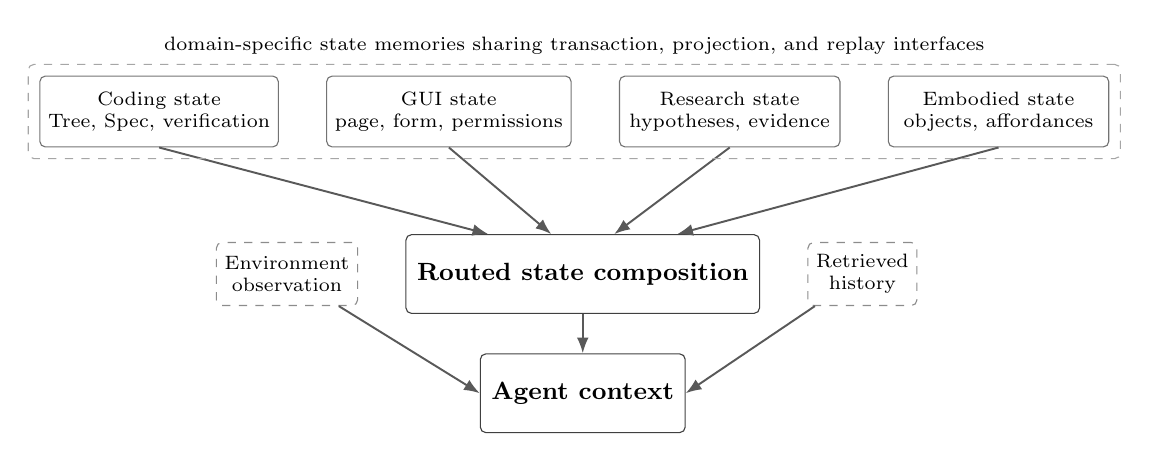
\begin{tikzpicture}[
  node distance=5mm and 6mm,
  memory/.style={draw=black!55, rounded corners=2pt, align=center,
                 minimum width=28mm, minimum height=9mm,
                 inner sep=3pt, font=\scriptsize},
  process/.style={draw=black!75, rounded corners=2pt, align=center,
                  minimum height=10mm, inner sep=4pt, font=\small\bfseries},
  evidence/.style={draw=black!45, dashed, rounded corners=2pt, align=center,
                   minimum height=8mm, inner sep=3pt, font=\scriptsize},
  arrow/.style={-{Latex[length=2mm]}, line width=0.7pt, draw=black!65}
]
  \node[memory] (code) {Coding state\\Tree, Spec, verification};
  \node[memory, right=of code] (gui) {GUI state\\page, form, permissions};
  \node[memory, right=of gui] (research) {Research state\\hypotheses, evidence};
  \node[memory, right=of research] (embodied) {Embodied state\\objects, affordances};

  \node[process, below=11mm of gui, xshift=17mm] (router)
    {Routed state composition};
  \node[evidence, left=of router] (observation) {Environment\\observation};
  \node[evidence, right=of router] (retrieval) {Retrieved\\history};
  \node[process, below=of router] (context) {Agent context};

  \draw[arrow] (code.south) -- ([xshift=-12mm]router.north);
  \draw[arrow] (gui.south) -- ([xshift=-4mm]router.north);
  \draw[arrow] (research.south) -- ([xshift=4mm]router.north);
  \draw[arrow] (embodied.south) -- ([xshift=12mm]router.north);
  \draw[arrow] (observation) -- (context.west);
  \draw[arrow] (router) -- (context);
  \draw[arrow] (retrieval) -- (context.east);

  \node[draw=black!35, dashed, rounded corners=2pt,
        fit=(code)(gui)(research)(embodied), inner sep=4pt,
        label={[font=\scriptsize]above:domain-specific state memories sharing
        transaction, projection, and replay interfaces}] {};
\end{tikzpicture}
\caption{A composable state-native memory architecture.  A router selects or
combines projections from domain-specific state models; those projections
complement rather than replace current environment observation and retrieval
memory.}
\label{fig:composable-state-memory}
\end{figure}

\section{Conclusion}

Long-horizon coding agents need more than a partial reading of implementation
outcomes plus retrieval of relevant past fragments.  They need a shared,
current, authoritative answer to where the project is, what the current branch
owns, which design governs it, how it reached its current state, and what
movement is admissible next.  \system treats this as a coordination-state
problem.

By combining an ordered Project Tree, dependency DAG, scope-owned Specs
and execution documents, protected lifecycle transitions, verification
evidence, deterministic Recall, and a compact event trajectory, \system makes
software development recoverable across context loss and agent handoffs.  The
method does not prescribe every action.  It supplies the durable state space
within which agents can inspect and modify code without repeatedly
reconstructing project coordination state from repository fragments and
conversation memory.

TreeWork is one coding-domain instance of a broader state-native memory
direction, not a universal schema.  Other long-horizon agents require different
action-relevant state spaces.  Future systems may therefore comprise a family
of domain-specific state models that share transaction, projection, and replay
interfaces, routing queries to or composing projections from several memories
according to the current environment and continuation problem.

\bibliographystyle{plainnat}
\bibliography{references}

\end{document}
